% Created 2021-12-07 ter 09:27
% Intended LaTeX compiler: pdflatex
\documentclass[xcolor=dvipsnames, 10pt, presentation,aspectratio=169]{beamer}
\usepackage[utf8]{inputenc}
\usepackage[T1]{fontenc}
\usepackage{graphicx}
\usepackage{grffile}
\usepackage{longtable}
\usepackage{wrapfig}
\usepackage{rotating}
\usepackage[normalem]{ulem}
\usepackage{amsmath}
\usepackage{textcomp}
\usepackage{amssymb}
\usepackage{capt-of}
\usepackage{hyperref}
\setbeamertemplate{footline}[frame number]
\usecolortheme[named=BrickRed]{structure}
\setbeamertemplate{navigation symbols}{}
\usepackage[american, english]{babel}
\usepackage{url} \urlstyle{sf}
\useinnertheme{circles}
\let\alert=\structure
\usepackage{wrapfig}
\usepackage{fancyvrb}
\newcommand{\bashcmd}[1]{\textcolor{White}{\colorbox{Sepia}{\texttt{#1}}}}
\usepackage{listings}
\lstset{
backgroundcolor=\color{red!10},
showstringspaces=false,
stringstyle=\ttfamily,
frame=single,
frameround=tttt,
mathescape=false
}
\logo{ 
\includegraphics[height=1cm,width=1cm,keepaspectratio]{logo_inf}    
\includegraphics[height=1cm,width=1cm,keepaspectratio]{logo_ufsm} }
\usetheme{Madrid}
\author{João Vicente Ferreira Lima}
\date{2021/2}
\title{Python System Programming}
\subtitle{Operating System Practice}
\institute[UFSM]{Universidade Federal de Santa Maria \\ \url{jvlima@inf.ufsm.br} \\ \url{http://www.inf.ufsm.br/~jvlima}}
\hypersetup{
 pdfauthor={João Vicente Ferreira Lima},
 pdftitle={Python System Programming},
 pdfkeywords={},
 pdfsubject={},
 pdfcreator={Emacs 24.5.1 (Org mode 8.3.4)}, 
 pdflang={English}}
\begin{document}

\maketitle
\frame<handout:0>
{
  \frametitle{Outline}
  \tableofcontents
}

\makeatletter
\AtBeginSubsection[]
{
  \frame<handout:0>
  {
    \frametitle{Outline}
    \tableofcontents[current,currentsubsection]
  }
}
\makeatother

\section{Fundamental concepts}
\label{sec:org251f05c}
\subsection{System calls}
\label{sec:org1b09d13}
\begin{frame}[label={sec:orge6fe0d0},fragile]{System calls}
 \begin{itemize}
\item A system call changes the processor state from user mode to kernel mode.
\item The number of system calls is fixed, and each system call has an
unique number.
\item Each system call may have a set of arguments that has information to
transfer to be transfered from user space to kernel space.
\end{itemize}

The system call steps are:
\begin{enumerate}
\item Calls a wrapper function in the C library.
\item The wrapper function copies the arguments to these registers.
\item The wrapper function copies the system call number into a specific
CPU register (\texttt{\%eax}).
\item The wrapper function executes a \emph{trap} instruction (\texttt{int 0x80}).
\item The kernel invokes its \emph{system\_call()}.
\item If the return value indicates an error, the wrapper function sets
the global variable \emph{errno}.
\end{enumerate}
\end{frame}

\begin{frame}[label={sec:org293cf65}]{System calls}
The Figure below illustrates the above steps for the \emph{execve()} system call.
\begin{center}
  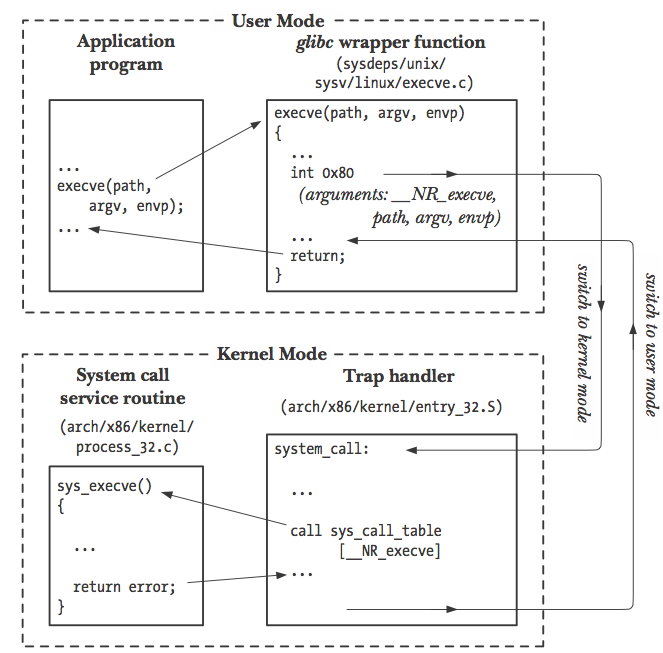
\includegraphics[scale=0.6]{systemCall.png}
\end{center}
\end{frame}

\subsection{Python system modules}
\label{sec:orgaa917e2}
\begin{frame}[label={sec:org6bb375c},fragile]{Python system modules}
 Most system-level calls are shipped in just two modules: \texttt{sys} and
\texttt{os}. \texttt{sys} exports components related to the Python \emph{interpreter} and \texttt{os}
contains variables and functions that map to the operating system.

Other related modules are:
\begin{description}
\item[{glob}] filename expansion.
\item[{socket}] network connections and IPC.
\item[{threading, queue}] running and synchronizing concurrent threads.
\item[{time, timeit}] system time details.
\item[{subprocess, multiprocessing}] launching and controlling parallel processes.
\item[{signal, select, shutil, tempfile, \emph{etc}}] system-related tasks
\end{description}
\end{frame}
\subsection{Time}
\label{sec:org4038672}
\begin{frame}[label={sec:orgb3c39ee},fragile]{Time}
 \lstset{language=Python,label= ,caption= ,captionpos=b,numbers=none}
\begin{lstlisting}
import time
from datetime import date

today = date.today()
print( "Today is: ", today)

timestamp = time.time()
print( "Timestamp now: ", timestamp )

time_today = date.fromtimestamp(timestamp)
print( "From timestamp:", time_today )
\end{lstlisting}

\begin{verbatim}
Today is:  2019-05-13
Timestamp now:  1557773061.429696
From timestamp: 2019-05-13
\end{verbatim}
\end{frame}
\begin{frame}[label={sec:orgb8f161c},fragile]{Time}
 \lstset{language=Python,label= ,caption= ,captionpos=b,numbers=none}
\begin{lstlisting}
import time
from datetime import date, datetime

t1 = time.time()
print("Sleeping 2 seconds...")
time.sleep(2)
t2 = time.time()

delta = datetime.fromtimestamp(t2-t1)
print("Seconds:", delta.second,
    "Microseconds:", delta.microsecond)
\end{lstlisting}

\begin{verbatim}
Sleeping 2 seconds...
Seconds: 2 Microseconds: 7270
\end{verbatim}
\end{frame}

\section{Processes}
\label{sec:orgc4d5347}
\subsection{Processes}
\label{sec:orgb16d6ca}
\begin{frame}[label={sec:orge8f40d8},fragile]{Introduction}
 The \texttt{os} module contains basic functions to run shell commands from
within Python scripts.  Two \texttt{os} functions allow scripts to run any
command line:
\begin{description}
\item[{\texttt{os.system}}] runs shell command
\item[{\texttt{os.popen}}] runs a shell command and connects to its input or
output.
\item[{\texttt{subprocess}}] intends to replace \texttt{os.system} and \texttt{os.spawn*}.
\end{description}
\end{frame}

\begin{frame}[label={sec:orgec5a489},fragile]{Current Working Directory}
 The CWD is the directory you where in when you typed this command, not
where the script resides.
On the other hand, Python automatically adds the identity of the
script's home directory to the front of the module search path in
order to import any other files.
\lstset{language=Python,label= ,caption= ,captionpos=b,numbers=none}
\begin{lstlisting}
import os
import sys

print('My os.getcwd: ' + os.getcwd())
print('My sys.path : ' + str(sys.path))
\end{lstlisting}

\begin{verbatim}
My os.getcwd: /Users/jvlima/pso/lectures
My sys.path : ['', '/usr/local/Cellar/python3/3.5.2_3/Frameworks/Python.framework/Versions/3.5/lib/python35.zip', '/usr/local/Cellar/python3/3.5.2_3/Frameworks/Python.framework/Versions/3.5/lib/python3.5', '/usr/local/Cellar/python3/3.5.2_3/Frameworks/Python.framework/Versions/3.5/lib/python3.5/plat-darwin', '/usr/local/Cellar/python3/3.5.2_3/Frameworks/Python.framework/Versions/3.5/lib/python3.5/lib-dynload', '/usr/local/lib/python3.5/site-packages']
\end{verbatim}
\end{frame}

\begin{frame}[label={sec:org21194fe},fragile]{Shell environment variables}
 Shell variables are available as \texttt{os.environ}, a Python dictionary-like
object with one entry per variable in the shell.
\lstset{language=Python,label= ,caption= ,captionpos=b,numbers=none}
\begin{lstlisting}
import os

print(os.environ.keys())
print(list(os.environ.keys()))
print('Variable TMPDIR is: ' + os.environ['TMPDIR'])
\end{lstlisting}

\begin{verbatim}
KeysView(environ({'XPC_FLAGS': '0x0', 'PWD': '/Users/jvlima/pso/lectures', 'SCRATCH': '/Users/jvlima', 'TERM': 'dumb', 'TERM_SESSION_ID': '3ECE587D-354D-4C48-BDCB-F7CE89511DB5', '_': '/usr/local/bin/python3', 'SECURITYSESSIONID': '186a8', 'DISPLAY': 'jvlima-imac.inf.ufsm.br', 'TERM_PROGRAM_VERSION': '387', 'LOGNAME': 'jvlima', 'TERM_PROGRAM': 'Apple_Terminal', '__CF_USER_TEXT_ENCODING': '0x1F5:0x0:0x0', 'PERL_MB_OPT': '--install_base "/Users/jvlima/perl5"', '__PYVENV_LAUNCHER__': '/usr/local/bin/python3', 'LC_CTYPE': 'UTF-8', 'SHELL': '/bin/bash', 'LANG': 'en_BR.UTF-8', 'SHLVL': '2', 'HOME': '/Users/jvlima', 'TMPDIR': '/var/folders/m6/d0jhl9fs19j82w4fck9qxs7m0000gn/T/', 'SSH_AUTH_SOCK': '/private/tmp/com.apple.launchd.f9J5Jk4Lgj/Listeners', 'XPC_SERVICE_NAME': '0', 'PATH': '/Users/jvlima/bin:/usr/local/bin:/usr/local/sbin:/usr/bin:/bin:/usr/sbin:/sbin:/usr/local/bin:/Library/TeX/texbin', 'PERL_MM_OPT': 'INSTALL_BASE=/Users/jvlima/perl5', 'Apple_PubSub_Socket_Render': '/private/tmp/com.apple.launchd.ZWqR5XU2KQ/Render', 'USER': 'jvlima'}))
['XPC_FLAGS', 'PWD', 'SCRATCH', 'TERM', 'TERM_SESSION_ID', '_', 'SECURITYSESSIONID', 'DISPLAY', 'TERM_PROGRAM_VERSION', 'LOGNAME', 'TERM_PROGRAM', '__CF_USER_TEXT_ENCODING', 'PERL_MB_OPT', '__PYVENV_LAUNCHER__', 'LC_CTYPE', 'SHELL', 'LANG', 'SHLVL', 'HOME', 'TMPDIR', 'SSH_AUTH_SOCK', 'XPC_SERVICE_NAME', 'PATH', 'PERL_MM_OPT', 'Apple_PubSub_Socket_Render', 'USER']
Variable TMPDIR is: /var/folders/m6/d0jhl9fs19j82w4fck9qxs7m0000gn/T/
\end{verbatim}
\end{frame}

\begin{frame}[label={sec:org32eac22},fragile]{Shell environment variables}
 To change or create variables, we can just assign a value like normal
dictionaries.
However, this new value is only visible to the enclosing shell
environment.
\lstset{language=Python,label= ,caption= ,captionpos=b,numbers=none}
\begin{lstlisting}
#!/usr/bin/env python3 
import os

print('Old value: ' + os.environ['USER'])
os.environ['USER'] = 'thing'
print('New value: ' + os.environ['USER'])
\end{lstlisting}

\begin{verbatim}
Old value: jvlima
New value: thing
\end{verbatim}
\end{frame}

\subsection{Running a shell command}
\label{sec:org9436adf}
\begin{frame}[label={sec:orgc7c2072},fragile]{Running a shell command}
 The \texttt{os.system} call lets Python scripts run any sort of command line
program. 
\lstset{language=Python,label= ,caption= ,captionpos=b,numbers=none}
\begin{lstlisting}
import os

ret = os.system('ls ..')
print('Return value: ' + str(ret))
\end{lstlisting}

\begin{verbatim}
LICENSE
README.org
assignments
lectures
scripts
Return value: 0
\end{verbatim}


The \texttt{os.system} returns the exit status, and redirects the command's
output in the session or standard output.
\end{frame}
\begin{frame}[label={sec:org1ed570a},fragile]{Communicating with shell commands}
 \texttt{os.popen} connects to the standard output or input of the command. If
we pass a \texttt{w} mode flag to \texttt{popen}, we connect to the command's input
stream.
\lstset{language=Python,label= ,caption= ,captionpos=b,numbers=none}
\begin{lstlisting}
import os

text = os.popen('ls ..').read()
print(text)

lines = os.popen('ls ..').readlines()
print(lines)
\end{lstlisting}

\begin{verbatim}
LICENSE
README.org
assignments
lectures
scripts

['LICENSE\n', 'README.org\n', 'assignments\n', 'lectures\n', 'scripts\n']
\end{verbatim}
\end{frame}

\subsection{\texttt{subprocess} module}
\label{sec:org0225122}
\begin{frame}[label={sec:org81d6e89},fragile]{\texttt{subprocess} module}
 As we mentioned before, the \texttt{subprocess} module intends to replate
several older modules and functions such as \texttt{os.system} and \texttt{os.spawn*}.

Running a shell command can be done using \texttt{run()} (recommended) or \texttt{call()}.
\lstset{language=Python,label= ,caption= ,captionpos=b,numbers=none}
\begin{lstlisting}
import subprocess

subprocess.run('date')
subprocess.run(['ls', '..'])
subprocess.run('hello.py', shell=True)
\end{lstlisting}

\begin{verbatim}
Wed Nov 16 14:39:46 BRST 2016
LICENSE
README.org
assignments
lectures
scripts
\end{verbatim}
\end{frame}

\begin{frame}[label={sec:org7ab8820},fragile]{\texttt{subprocess} module}
 Two things must be noted here:
\begin{enumerate}
\item The second command received a list in which the first element is
the command and the second its arguments.
\item The \texttt{shell=True} argument. On Unix-like platforms, when \texttt{shell} is
\texttt{False}, the program command line is run directly by \texttt{os.execvp}. If
this argument is \texttt{True}, the command is run through a shell instead.
\end{enumerate}
\end{frame}

\subsection{Forking processes}
\label{sec:orge775c52}
\begin{frame}[label={sec:org13ef7ed},fragile]{Forking processes}
 \lstset{language=Python,label= ,caption= ,captionpos=b,numbers=none}
\begin{lstlisting}
import os

def child():
  print('Hello from child', os.getpid())
  os._exit(0)

def parent():
  while True:
    newpid = os.fork()
    if newpid == 0:
      child()
    else:
      print('Hello from parent', os.getpid(), newpid)
    if input() == 'q':
      break
parent()
\end{lstlisting}
\end{frame}
\begin{frame}[label={sec:orgd675987},fragile]{Forking processes}
 \lstset{language=Python,label= ,caption= ,captionpos=b,numbers=none}
\begin{lstlisting}
import os, time

def counter(count):
  for i in range(count):
    time.sleep(1)
    print('[%s] => %s' % (os.getpid(), i))

for i in range(5):
  pid = os.fork()
  if pid != 0:
    print('Process %s spawned' % pid)
  else:
    counter(5)
    os._exit(0)

print('Main process exiting.')
\end{lstlisting}
\end{frame}
\begin{frame}[label={sec:orgaeeb646},fragile]{Fork}
 \lstset{language=Python,label= ,caption= ,captionpos=b,numbers=none}
\begin{lstlisting}
import os

parm = 0
while True:
  parm += 1
  pid = os.fork()
  if pid == 0:
    os.execlp('python', 'python', 'child.py', str(parm))
    assert False, 'error starting program'
  else:
    print('Child is', pid)
    if input() == 'q':
      break
\end{lstlisting}
\end{frame}
\begin{frame}[label={sec:orgdd8ec73},fragile]{Exec}
 \lstset{language=Python,label= ,caption= ,captionpos=b,numbers=none}
\begin{lstlisting}
import os
import sys

print('Hello from child', os.getpid(), sys.argv[1])
\end{lstlisting}

A list of \texttt{os.exec} variants are:
\begin{verbatim}
os.execv(program, commandlinesequence)
os.execl(program, cmdarg1, cmdarg2, ... cmdargN)
os.execlp
os.execvp
os.execvpe
os.execlpe
\end{verbatim}
\end{frame}

\subsection{Threads}
\label{sec:org062082f}
\begin{frame}[label={sec:org2532113},fragile]{Threading}
 The \texttt{threading} module uses the \texttt{\_thread} module (lower-level interface)
to implement a higher-level interface based on objects and classes.

\lstset{language=Python,label= ,caption= ,captionpos=b,numbers=none}
\begin{lstlisting}
import threading
\end{lstlisting}
\end{frame}
\begin{frame}[label={sec:orgc71523b},fragile]{Threading}
 This example demostrates a threading class (\texttt{MyThead}):
\lstset{language=Python,label= ,caption= ,captionpos=b,numbers=none}
\begin{lstlisting}
import threading

class MyThread(threading.Thread):
  def __init__(self, myId, count, mutex):
    self.myId = myId
    self.count = count
    self.mutex = mutex
    threading.Thread.__init__(self)

  def run(self):
    for i in range(self.count):
      with self.mutex:
        print('[%s] => %s' % (self.myId, i))
\end{lstlisting}
\end{frame}
\begin{frame}[label={sec:org1fef440},fragile]{Threading}
 \lstset{language=Python,label= ,caption= ,captionpos=b,numbers=none}
\begin{lstlisting}
stdoutmutex = threading.Lock()
threads = []

for i in range(10):
  thread = MyThread(i, 10, stdoutmutex)
  thread.start()
  threads.append(thread)

for thread in threads:
  thread.join()

print('Main thread exiting.')
\end{lstlisting}
\end{frame}
\begin{frame}[label={sec:orgab126f6},fragile]{Threading}
 \begin{verbatim}
[0] => 0
[0] => 1
[0] => 2
[0] => 3
[0] => 4
[0] => 5
[0] => 6
[0] => 7
[0] => 8
[0] => 9
[1] => 0
[1] => 1
[1] => 2
[1] => 3
[1] => 4
[1] => 5
[1] => 6
[1] => 7
[1] => 8
[1] => 9
[2] => 0
[2] => 1
[2] => 2
[2] => 3
[2] => 4
[2] => 5
[2] => 6
[2] => 7
[2] => 8
[2] => 9
[3] => 0
[3] => 1
[3] => 2
[3] => 3
[3] => 4
[3] => 5
[3] => 6
[3] => 7
[3] => 8
[3] => 9
[4] => 0
[4] => 1
[4] => 2
[4] => 3
[4] => 4
[4] => 5
[4] => 6
[4] => 7
[4] => 8
[4] => 9
[5] => 0
[5] => 1
[5] => 2
[5] => 3
[5] => 4
[5] => 5
[5] => 6
[5] => 7
[5] => 8
[5] => 9
[6] => 0
[6] => 1
[6] => 2
[6] => 3
[6] => 4
[6] => 5
[6] => 6
[6] => 7
[6] => 8
[6] => 9
[7] => 0
[7] => 1
[7] => 2
[7] => 3
[7] => 4
[7] => 5
[7] => 6
[7] => 7
[7] => 8
[7] => 9
[8] => 0
[8] => 1
[8] => 2
[8] => 3
[8] => 4
[8] => 5
[8] => 6
[8] => 7
[8] => 8
[8] => 9
[9] => 0
[9] => 1
[9] => 2
[9] => 3
[9] => 4
[9] => 5
[9] => 6
[9] => 7
[9] => 8
[9] => 9
Main thread exiting.
\end{verbatim}
\end{frame}
\begin{frame}[label={sec:org030ce1a},fragile]{Threading}
 Your thread class do not necessarily have to subclass \texttt{Thread}. The
thread's target in \texttt{threading} may be any type of \emph{callable object}.
\lstset{language=Python,label= ,caption= ,captionpos=b,numbers=none}
\begin{lstlisting}
import threading

class Power:
    def __init__(self, i):
        self.i = i
    def action(self):
        print(self.i ** 32)

obj = Power(2)
threading.Thread(target=obj.action).start()
\end{lstlisting}

\begin{verbatim}
4294967296
\end{verbatim}
\end{frame}
\begin{frame}[label={sec:org74f105f},fragile]{Threading}
 Global variables can require coordination if concurrent updates are
possible, such as:
\lstset{language=Python,label= ,caption= ,captionpos=b,numbers=none}
\begin{lstlisting}
import threading
import time

count = 0

def adder():
    global count
    count = count + 1
    time.sleep(0.5)
    count = count + 1
\end{lstlisting}
\end{frame}
\begin{frame}[label={sec:org81dc2a6},fragile]{Threading}
 \lstset{language=Python,label= ,caption= ,captionpos=b,numbers=none}
\begin{lstlisting}
threads = []
for i in range(100):
    thread = threading.Thread(target=adder, args=())
    thread.start()
    threads.append(thread)

for thread in threads:
    thread.join()
print(count)
\end{lstlisting}

\begin{verbatim}
200
\end{verbatim}
\end{frame}
\begin{frame}[label={sec:org1172f23},fragile]{Threading}
 This code clearly has a race condition on the update of \texttt{count} global
variable. To avoid this race, we need to add a lock to synchronize the
updates:
\lstset{language=Python,label= ,caption= ,captionpos=b,numbers=none}
\begin{lstlisting}
import threading
import time

count = 0

def adder(addlock):
    global count
    with addlock:
        count = count + 1
    time.sleep(0.5)
    with addlock:
        count = count + 1
\end{lstlisting}
\end{frame}
\begin{frame}[label={sec:org7b848e1},fragile]{Threading}
 \lstset{language=Python,label= ,caption= ,captionpos=b,numbers=none}
\begin{lstlisting}
addlock = threading.Lock()
threads = []
for i in range(100):
    thread = threading.Thread(target=adder, args=(addlock,))
    thread.start()
    threads.append(thread)

for thread in threads:
    thread.join()
print(count)
\end{lstlisting}

\begin{verbatim}
200
\end{verbatim}
\end{frame}

\begin{frame}[label={sec:orged5c2fd},fragile]{Queue}
 The \texttt{queue} module provides a standard queue data structure (FIFO),
in which items are added on one end and removed from the other.
The queue object is automatically controlled with thread lock acquire
and release operations.

In this example, the program runs two producers and two consumers
(five threads including the main one). Note that consumers threads are
set to be \emph{daemon} threads. The entire program exits when only deamon
threads are left. Producer threads end with a \emph{join} at the end.
\end{frame}
\begin{frame}[label={sec:orgc912d80},fragile]{Queue}
 \lstset{language=Python,label= ,caption= ,captionpos=b,numbers=none}
\begin{lstlisting}
import threading
import queue
import time

nconsumers = 2
nproducers = 2
nmessages = 4

safeprint = threading.Lock()
dataQueue = queue.Queue()
\end{lstlisting}
\end{frame}
\begin{frame}[label={sec:orgc281341},fragile]{Producer/consumer}
 \lstset{language=Python,label= ,caption= ,captionpos=b,numbers=none}
\begin{lstlisting}
def producer(idnum):
    for msg in range(nmessages):
        time.sleep(idnum)
        dataQueue.put('[producer id=%d, count=%d]' % 
                      (idnum, msg))

def consumer(idnum):
    while True:
        time.sleep(0.1)
        try:
            data = dataQueue.get(block=False)
        except queue.Empty:
            pass
        else:
            with safeprint:
                print('consumer', idnum,
                      'got =>', data)
\end{lstlisting}
\end{frame}
\begin{frame}[label={sec:org7276104},fragile]{Producer/consumer}
 \lstset{language=Python,label= ,caption= ,captionpos=b,numbers=none}
\begin{lstlisting}
if __name__ == '__main__':
    for i in range(nconsumers):
        thread = threading.Thread(target=consumer,
                                  args=(i,))
        thread.daemon = True # else cannot exit
        thread.start()

    threads = []        
    for i in range(nproducers):
        thread = threading.Thread(target=producer,
                                  args=(i,))
        thread.start()
        threads.append(thread)

    for thread in threads:
        thread.join()
\end{lstlisting}
\end{frame}
\begin{frame}[label={sec:orgeb15a4c},fragile]{Producer/consumer}
 \begin{verbatim}
consumer 0 got => [producer id=0, count=0]
consumer 1 got => [producer id=0, count=1]
consumer 0 got => [producer id=0, count=2]
consumer 1 got => [producer id=0, count=3]
consumer 0 got => [producer id=1, count=0]
consumer 0 got => [producer id=1, count=1]
consumer 0 got => [producer id=1, count=2]
\end{verbatim}
\end{frame}

\begin{frame}[label={sec:org63d9b30},fragile]{Other synchronization objects}
 \begin{description}
\item[{\texttt{threading.RLock}}] reentrant lock.
\item[{\texttt{threading.Condition(lock=None)}}] condition variable.
\item[{\texttt{threading.Semaphore(value=1)}}] semaphore.
\item[{\texttt{threading.Event}}] one thread signals an event and other threads wait for it.
\end{description}
\end{frame}
\subsection{Interprocess communication}
\label{sec:orgf364fb8}
\begin{frame}[label={sec:org03307ce}]{Pipes}
Pipes are implemented by the operating system and made available in
the Python standard library.  Pipes are unidirectional channels.

\begin{block}{Anonymous and named pipes}
There are \emph{anonymous} and \emph{named} pipes. Named pipes (or fifos) are
external files. By contrast, anonymous pipes exist only within
processes and are tipically used in conjunction with process \emph{forks}.
\end{block}
\end{frame}
\begin{frame}[label={sec:orgc67cb90},fragile]{Anonymous Pipes}
 This example forks itself and creates a pipe. The \texttt{os.pipe} call returns
a tuple of two file descriptors, representing the input and output
sides of the pipe.
\lstset{language=Python,label= ,caption= ,captionpos=b,numbers=none}
\begin{lstlisting}
import os, time

def child(pipeout):
    zzz = 0
    while True:
        # make parent wait
        time.sleep(zzz)
        # pipes are binary bytes
        msg = ('Spam %03d' % zzz).encode()
        # send to parent
        os.write(pipeout, msg)
        # goto 0 after 4
        zzz = (zzz+1) % 5
\end{lstlisting}
\end{frame}
\begin{frame}[label={sec:orgd227b8b},fragile]{Anonymous Pipes}
 \lstset{language=Python,label= ,caption= ,captionpos=b,numbers=none}
\begin{lstlisting}
def parent():
    # make 2-ended pipe
    pipein, pipeout = os.pipe()
    # copy this process
    if os.fork() == 0:
        child(pipeout)
    else:
        # in parent, listen to pipe
        while True:
            # blocks until data sent
            line = os.read(pipein, 32)
            print('Parent %d got [%s] at %s' %
                  (os.getpid(), line, time.time()))

parent()
\end{lstlisting}
\end{frame}
\begin{frame}[label={sec:orga26e804},fragile]{Anonymous Pipes}
 \begin{verbatim}
Parent 79486 got [b'Spam 000'] at 1479696342.063272
Parent 79486 got [b'Spam 001'] at 1479696343.063545
Parent 79486 got [b'Spam 002'] at 1479696345.065001
Parent 79486 got [b'Spam 003'] at 1479696348.066442
Parent 79486 got [b'Spam 004'] at 1479696352.067562
Parent 79486 got [b'Spam 000'] at 1479696352.067668
Parent 79486 got [b'Spam 001'] at 1479696353.068904
Parent 79486 got [b'Spam 002'] at 1479696355.070184
Parent 79486 got [b'Spam 003'] at 1479696358.071641
Parent 79486 got [b'Spam 004Spam 000'] at 1479696362.073227
Parent 79486 got [b'Spam 001'] at 1479696363.074522
Parent 79486 got [b'Spam 002'] at 1479696365.075826
Parent 79486 got [b'Spam 003'] at 1479696368.077408
Parent 79486 got [b'Spam 004Spam 000'] at 1479696372.078836
Parent 79486 got [b'Spam 001'] at 1479696373.079927
\end{verbatim}
\end{frame}

\begin{frame}[label={sec:orgf66a362},fragile]{Named pipes (Fifos)}
 \begin{block}{Named pipes}
Named pipes are external files to any particular program. Once a named
pipe file is create, clients open it by name and read and write data
using normal file operations.
\end{block}

In this example, a named pipe is created with the \texttt{os.mkfifo}
call. Because the fifo exists independently of both parent and child,
there is no reason to fork here.
\end{frame}
\begin{frame}[label={sec:org4ac24ad},fragile]{Named pipes (Fifos)}
 \lstset{language=Python,label= ,caption= ,captionpos=b,numbers=none}
\begin{lstlisting}
import os, time, sys
fifoname = '/tmp/pipefifo' 

def child():
    # open fifo pipe file as fd
    pipeout = os.open(fifoname, os.O_WRONLY)
    zzz = 0
    while True:
        time.sleep(zzz)
        # binary as opened here
        msg = ('Spam %03d\n' % zzz).encode()
        os.write(pipeout, msg)
        zzz = (zzz+1) % 5
\end{lstlisting}
\end{frame}
\begin{frame}[label={sec:org2e55327},fragile]{Named pipes (fifos)}
 \lstset{language=Python,label= ,caption= ,captionpos=b,numbers=none}
\begin{lstlisting}
def parent():
    # open fifo as text file object
    pipein = open(fifoname, 'r') 
    while True:
        # blocks until data sent
        line = pipein.readline()[:-1] 
        print('Parent %d got "%s" at %s' % 
              (os.getpid(), line, time.time()))

if __name__ == '__main__':
    if not os.path.exists(fifoname):
        os.mkfifo(fifoname) 
    if len(sys.argv) == 1:
        parent()          
    else: 
        child()
\end{lstlisting}
\end{frame}

\begin{frame}[label={sec:org6eb55a7},fragile]{Named pipes (Fifos)}
 Execute the parent typing:
\lstset{language=sh,label= ,caption= ,captionpos=b,numbers=none}
\begin{lstlisting}
python pipefifo.py
Parent 80553 got "Spam 000" at 1479700554.835515
Parent 80553 got "Spam 001" at 1479700555.840781
Parent 80553 got "Spam 002" at 1479700557.845987
Parent 80553 got "Spam 003" at 1479700560.84998
Parent 80553 got "Spam 004" at 1479700564.855003
Parent 80553 got "Spam 000" at 1479700564.855088
Parent 80553 got "Spam 001" at 1479700565.859777
.....
\end{lstlisting}
Execute the child:
\lstset{language=sh,label= ,caption= ,captionpos=b,numbers=none}
\begin{lstlisting}
python pipefifo.py -child
\end{lstlisting}
\end{frame}

\section{Other \texttt{os} module exports}
\label{sec:orgb51522d}
\subsection{Other \texttt{os} module exports}
\label{sec:orga5ea30a}
\begin{frame}[label={sec:orga7f7c5d},fragile]{Other \texttt{os} module exports}
 \begin{description}
\item[{\texttt{os.environ}}] manipulates environment variables.
\item[{\texttt{os.fork}}] spawns a new child process.
\item[{\texttt{os.pipe}}] communicates between programs.
\item[{\texttt{os.execlp}}] starts new programs.
\item[{\texttt{os.spawnv}}] starts new programs with lower-level control.
\item[{\texttt{os.open}}] opens a low-level descriptor file.
\item[{\texttt{os.mkdir}}] creates a new directory.
\item[{\texttt{os.mkfifo}}] creates a new named pipe.
\item[{\texttt{os.stat}}] fetches low-level file information.
\item[{\texttt{os.remove}}] deletes a file by its pathname.
\item[{\texttt{os.walk}}] applies a function or loop body to all parts of an entire
directory tree.
\end{description}
\end{frame}
\begin{frame}[label={sec:org7734c19}]{}
\end{frame}
\end{document}